\documentclass[a4paper, 11pt]{book}
\usepackage{/home/nora/Documents/Enseignement/Prepa/bpep/fichiers_utiles/preambule}

\makeatletter
\renewcommand{\@chapapp}{Kh\^olles MPSI3 -- semaine}
\renewcommand\thechapter{6}
\makeatother

% \toggletrue{student}
% \toggletrue{corrige}

\begin{document}

\settype{enon}
\settype{solu}

\chapter{Sujet 1\siCorrige{\!\!-- corrig\'e}}

\resetQ
\subimport{/home/nora/Documents/Enseignement/Prepa/bpep/exercices/TD/masse_astronaute_ISS/}{sujet.tex}


\chapter{Sujet 2\siCorrige{\!\!-- corrigé}}

\resetQ
\subimport{/home/nora/Documents/Enseignement/Prepa/bpep/exercices/Colle/energie_oscillateur_harmonique/}{sujet.tex}


\chapter{Sujet 3\siCorrige{\!\!-- corrigé}}

\resetQ
\subimport{/home/nora/Documents/Enseignement/Prepa/bpep/exercices/Colle/vibration_molecule/}{sujet.tex}

\chapter{Sujet 4\siCorrige{\!\!-- corrigé}}

\resetQ
\subimport{/home/nora/Documents/Enseignement/Prepa/bpep/exercices/TD/longueur_equilibre/}{sujet.tex}

\resetQ
\subimport{/home/nora/Documents/Enseignement/Prepa/bpep/exercices/TD/oscillateur_harmonique_et_approche_energetique/}{sujet.tex}

\chapter{Sujet 5\siCorrige{\!\!-- corrigé}}
\resetQ
\section{Circuit de \textsc{Wien}}

\begin{minipage}{0.60\linewidth}
	On réalise le montage suivant. On ferme l'interrupteur à l'instant $t =0$,
	$C$ traversé par $i'$ étant initialement chargé et $C$ traversé par $i$
	étant initialement déchargé.\smallbreak
	On pose $\tau = RC$. Données~: $R = \SI{10}{k\ohm}$ et $C = \SI{0.1}{\micro
			F}$.
\end{minipage}
\begin{minipage}{0.40\linewidth}
	\centering
	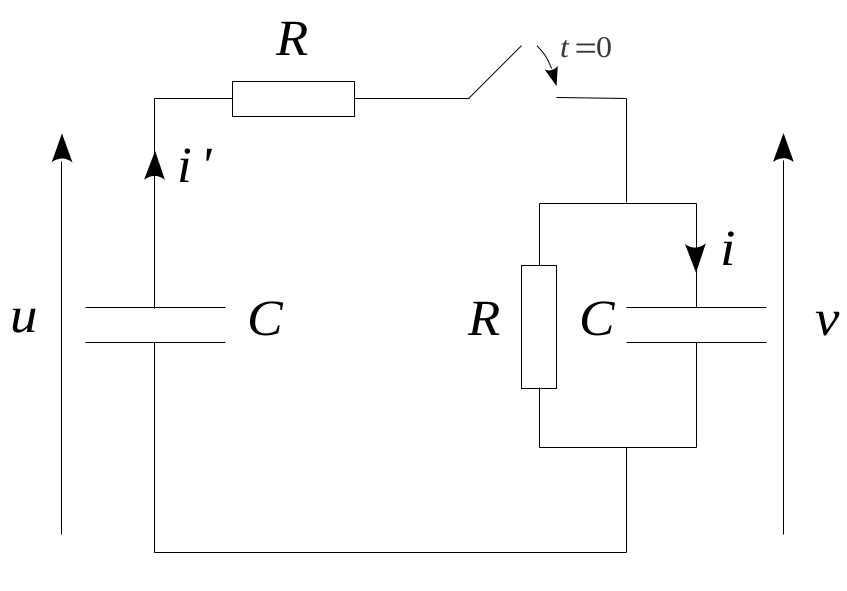
\includegraphics[width=\linewidth]{wien}
\end{minipage}

\QR{%
	À partir de considérations physiques, préciser les valeurs de la tension $v$
	lorsque $t = 0$ et $t = \infty$.
}{%
	Le condensateur de tension $v$ est indiqué être initialement déchargé, on a
	donc $v(0^-) = 0$. Comme un condensateur est de tension continue, on a donc
	\fbox{$v(0^+) = 0$}. De plus, à $t \longrightarrow \infty$, les deux
	condensateurs seront forcément déchargés à cause des résistances dissipant
	l'énergie, il ne peut y avoir conservation~: il seront donc équivalent à des
	interrupteurs ouverts, et on aura donc notamment \fbox{$v(\infty) = 0$}.
}%

\QR{%
	Établir l'équation différentielle du second ordre dont la tension $v$ est
	solution.
}{%
	Avec une loi des mailles, on a
	\[ u = v+Ri'\]
	Or, la RCT du condensateur de gauche \textbf{en convention générateur} est
	\[i' = -C \dv{u}{t} \Rightarrow i' = -C \dv{v}{t} - RC \dv{i'}{t}\]
	On a donc une équation avec $\dv{v}{t}$. On cherche donc à exprimer $i'$ en
	fonction de $v$, ce que l'on fait avec la loi des nœuds et les RCT du
	condensateur de droite $i = C \dv{v}{t}$ et de la résistance $R(i'-i) = v$~:
	\begin{equation}\label{eq:wieni}
		i' = i + \frac{v}{R} \Leftrightarrow i' = C \dv{v}{t} + \frac{v}{R}
	\end{equation}
	En combinant les deux, on a
	\begin{gather*}
		C \dv{v}{t} + \frac{v}{R} =
		-C \dv{v}{t} - RC \dv{}{t} \left( C \dv{v}{t} + \frac{v}{R} \right)
		\Leftrightarrow
		C \dv{v}{t} + \frac{v}{R} =
		-C \dv{v}{t} - RC^2 \dv[2]{v}{t} - C \dv{v}{t}\\
		\Leftrightarrow
		\dv[2]{v}{t} + \frac{3}{RC} \dv{v}{t} + \frac{v}{(RC)^2} = 0
		\Leftrightarrow
		\boxed{\dv[2]{v}{t} + \frac{3}{\tau} \dv{v}{t} + \frac{v}{\tau^2} = 0}
	\end{gather*}
}%

\QR{%
	En déduire l'expression de $v(t)$ sans chercher à déterminer les
	constantes d'intégration.
}{%
	On écrit l'équation caractéristique de discriminant $\Delta$~:
	\begin{gather*}
		r^2 + \frac{3}{\tau}r + \frac{1}{\tau^2} = 0 \Rightarrow \Delta =
		\frac{9}{\tau^2} - \frac{4}{\tau^2} = \frac{5}{\tau^2} > 0\\
		\Longrightarrow r_\pm = - \frac{3}{2\tau} \pm \frac{\sqrt{5}}{2\tau} < 0
	\end{gather*}
	On a donc un régime apériodique, dont les solutions générales sont
	\[\boxed{v(t) = A\exr^{r_+t} + B\exr^{r_-t}}\]
}%

\QR{%
	Donner l'allure du graphe correspondant à $v(t)$.
}{%
	\begin{minipage}{0.49\linewidth}
		Le condensateur est initialement chargé. Soit $E$ sa tension initiale.
		On utilise l'équation~\ref{eq:wieni} pour trouver que $\dv{v}{t} (0) =
			\frac{i' (0)}{C}$, sachant qu'à $t = 0$ le circuit est équivalent à un
		circuit $RC$ en décharge et qu'on a donc $i'(0) = E/R$. On trouve ainsi
		\[\boxed{\dv{v}{t} (0) = \frac{E}{\tau}}\]
		En finissant la détermination des constantes d'intégration, on trouve
		\begin{equation*}
			\boxed{v(t) = \frac{E}{\tau(r_+ - r_-)}
				\left[ \exr^{r_+t} - \exr^{r_-t} \right]}
		\end{equation*}
		\hfill
	\end{minipage}
	\begin{minipage}{0.49\linewidth}
		\begin{center}
			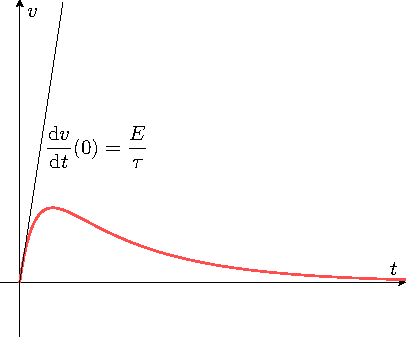
\includegraphics[width=\linewidth]{wien_carac}
		\end{center}
	\end{minipage}
}%
\end{document}

\end{document}
